
\appendix
\section{Code for Algorithm~\ref{alg:poldec}} \label{app:poldec.m}
\begin{lstlisting}
function [X, H, its, delta, Rk] = poldec(A, TOL)
%POLDEC Polar decomposition.
% [U, H, ITS, DELTA, RK] = poldec(A) computes the polar decomposition 
% A = U*H of the square, nonsingular matrix A. ITS is the number of
% iterations for convergence. DELTA is the relative error between 
% successive iterations. RK is the norm(X'X - I) at each iteration.
[n,m] = size(A);
if n ~= m
    error('Input matrix is not square!');
end
if nargin == 2
    err = TOL;
else
    err = eps("double");
end
I = eye(n); term_tol = sqrt(2*err)*sqrt(n); maxiter = 1e6;
X = A; switched = false; 
delta = zeros(maxiter,1); Rk = zeros(maxiter,1);
for its = 1:maxiter
    % check if switch to Newton Schulz
    Rk(its) = norm(X'*X - I,inf);
    if Rk(its) <= 0.6
        switched = true;
    end
    % apply appropriate iterations
    if switched % Newton Schulz iteration
        tmp = X;
        X = 1.5*X - 0.5*X*(X'*X);
        delta(its+1) = norm(X - tmp,inf)/norm(X,inf); % store error
        % termination condition
        if delta(its+1) < term_tol || (delta(its+1) > delta(its)/(2) && its ~= 1)
            break;
        end
    else % Newton iteration
        tmp = X;
        X = 0.5*(inv(X)' + X);
        delta(its+1) = norm(X - tmp,inf)/norm(X,inf); % store error
    end
end
H = 0.5*(X'*A + A'*X); % construct H
end
\end{lstlisting}
\newpage 
\section{Testing Routine} \label{app:testingroutine}
\begin{lstlisting}
% testing routine
clc; clear; close all; format short e
rng(1);
print = true;
A = hadamard(8); A_mp = mp(A, 34);
term_tol = sqrt(2*eps("double"))*sqrt(size(A,1));
[U_d,H_d,its_d,del_d,Rk_d] = poldec(A);
[U_q,H_q,its_q,del_q,Rk_q] = poldec(A,5e-34);
% printing results
fprintf("Condition number = %.4d\n", cond(A,inf));
fprintf("Iteration required = %d\n", its_d);
tmp1 = norm(A - U_d*H_d, inf)/norm(A,inf);
fprintf("norm(A-UH)/norm(A) = %.4d\n", tmp1);
tmp2 = norm(U_d'*U_d - eye(size(A,1)));
fprintf("norm(U'*U-I) = %.4d\n", tmp2);
tmp3 = norm(U_d - U_q,inf);
fprintf("norm(U-U_ref) = %.4d\n", tmp3);

if print 
    figure('Renderer', 'painters', 'Position', [200 200 900 900])
    semilogy(1:its_d, del_d(2:its_d+1),'-^k', 'LineWidth', 2);
    hold on;
    semilogy(1:its_d, Rk_d(1:its_d),'-^r', 'LineWidth', 2);
    semilogy(1:its_d, ones(1,its_d).*term_tol, '--b', 'LineWidth', 2);
    legend("$\|X_{k+1}-X_{k}\|_{\infty}/\|X_{k+1}\|_{\infty}$", ...
        "$\|X_k^*X_k - I\|_{\infty}$", ...
        "Terminate tolerance", ...
        "Location","southwest", ...
        "Interpreter", "latex");
    xlabel("Iteration");
    axis square;
    set(gca, "FontSize", 30)    
end
\end{lstlisting}

\section{Routine for Matrix Square Root}\label{app:matrix-squareroot}
\begin{lstlisting}
function H = polsqrt(A)
%POLSQRT Matrix square root using polar decomposition.
% H = poldec(A) computes the matrix square root of the symmetric 
% positive definite matrix A, such that norm(H^2 - A) is small.
R = chol(A);
[~,H] = poldec(R);
end
\end{lstlisting}

\section{Figures}\label{app:figs}

\begin{figure}[H]
    \centering
    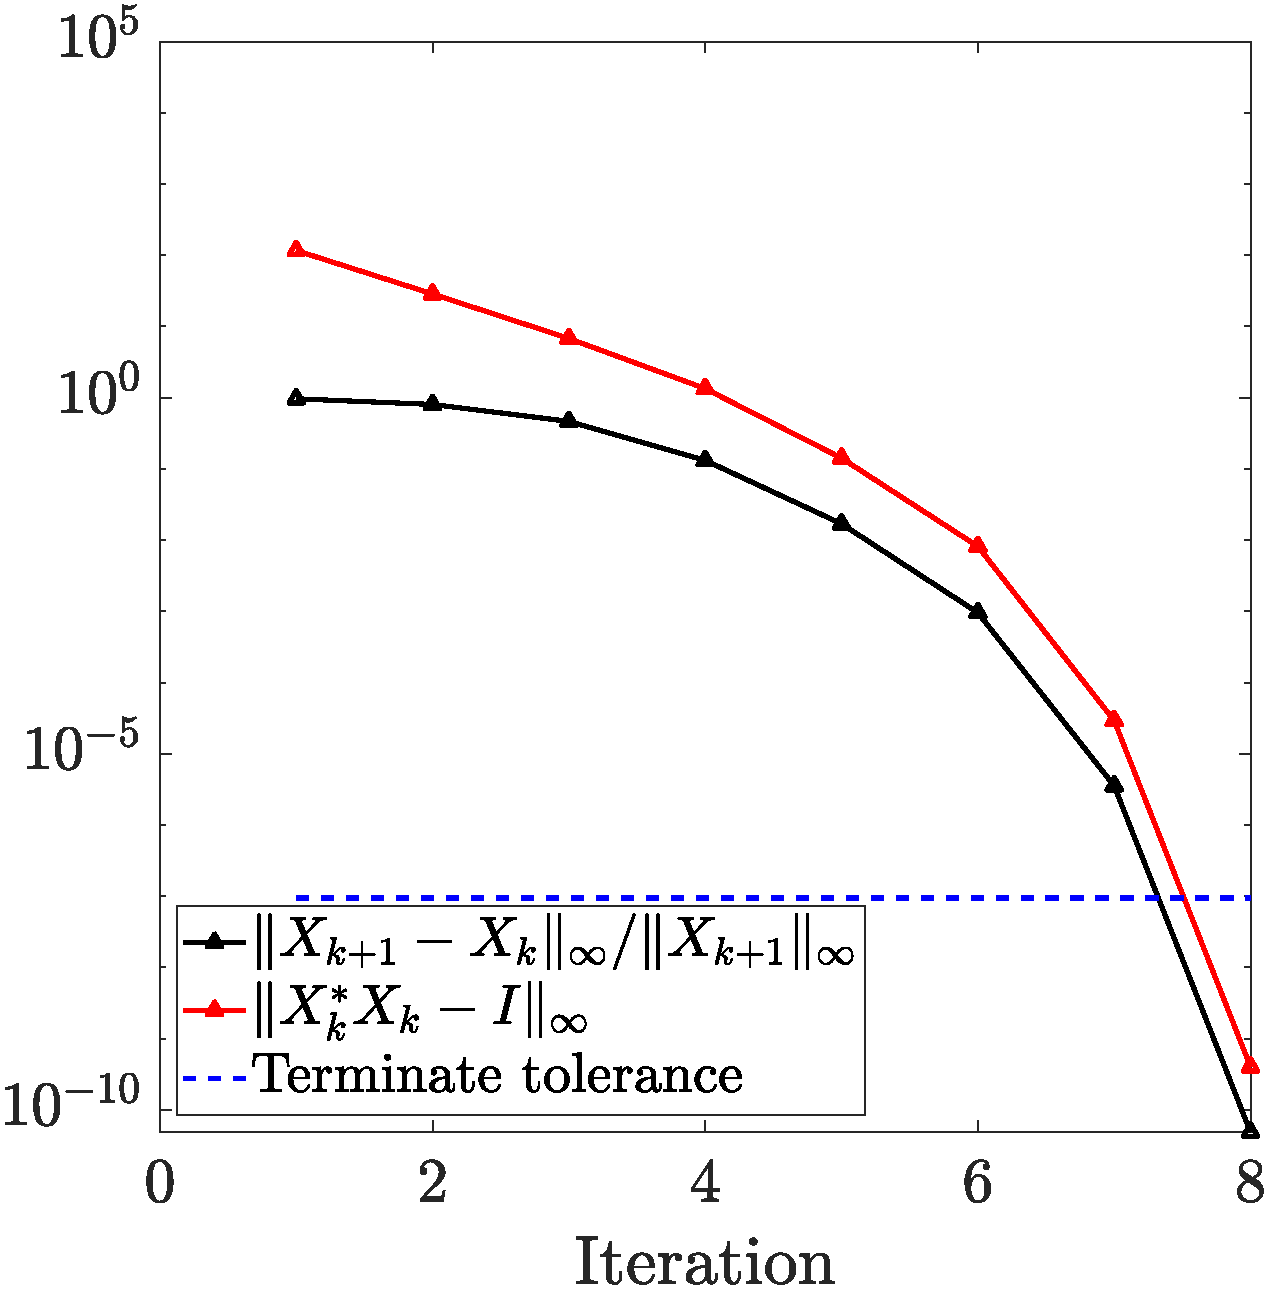
\includegraphics[width=0.59\textwidth]{../code/randn20.pdf}
    \caption{Behaviour of $\gnorm{X_{k+1} - X_{k}}_\infty/\gnorm{X_{k+1}}_\infty$ and $\gnorm{X\ctp X - I}_\infty$ with respect to the iteration when applying \inline{poldec} on \inline{randn(20)}.}
\end{figure}

\begin{figure}[H]
    \centering
    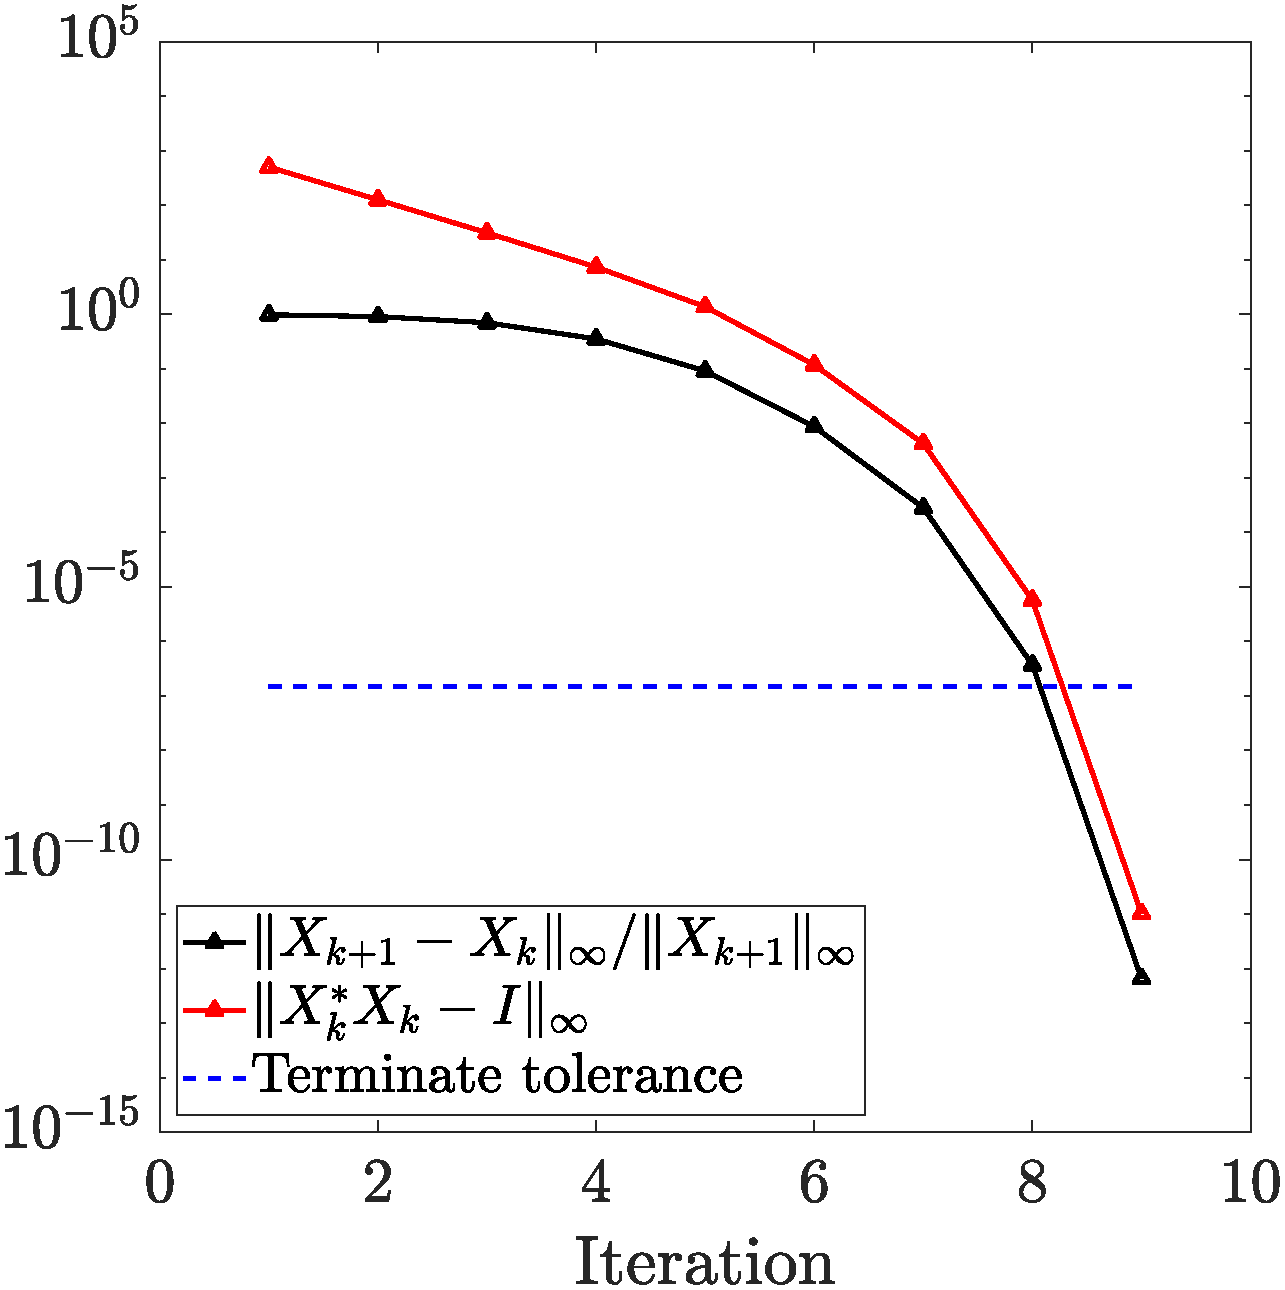
\includegraphics[width=0.6\textwidth]{../code/randn50.pdf}
    \caption{Behaviour of $\gnorm{X_{k+1} - X_{k}}_\infty/\gnorm{X_{k+1}}_\infty$ and $\gnorm{X\ctp X - I}_\infty$ with respect to the iteration when applying \inline{poldec} on \inline{randn(50)}.}
\end{figure}

\begin{figure}[H]
    \centering
    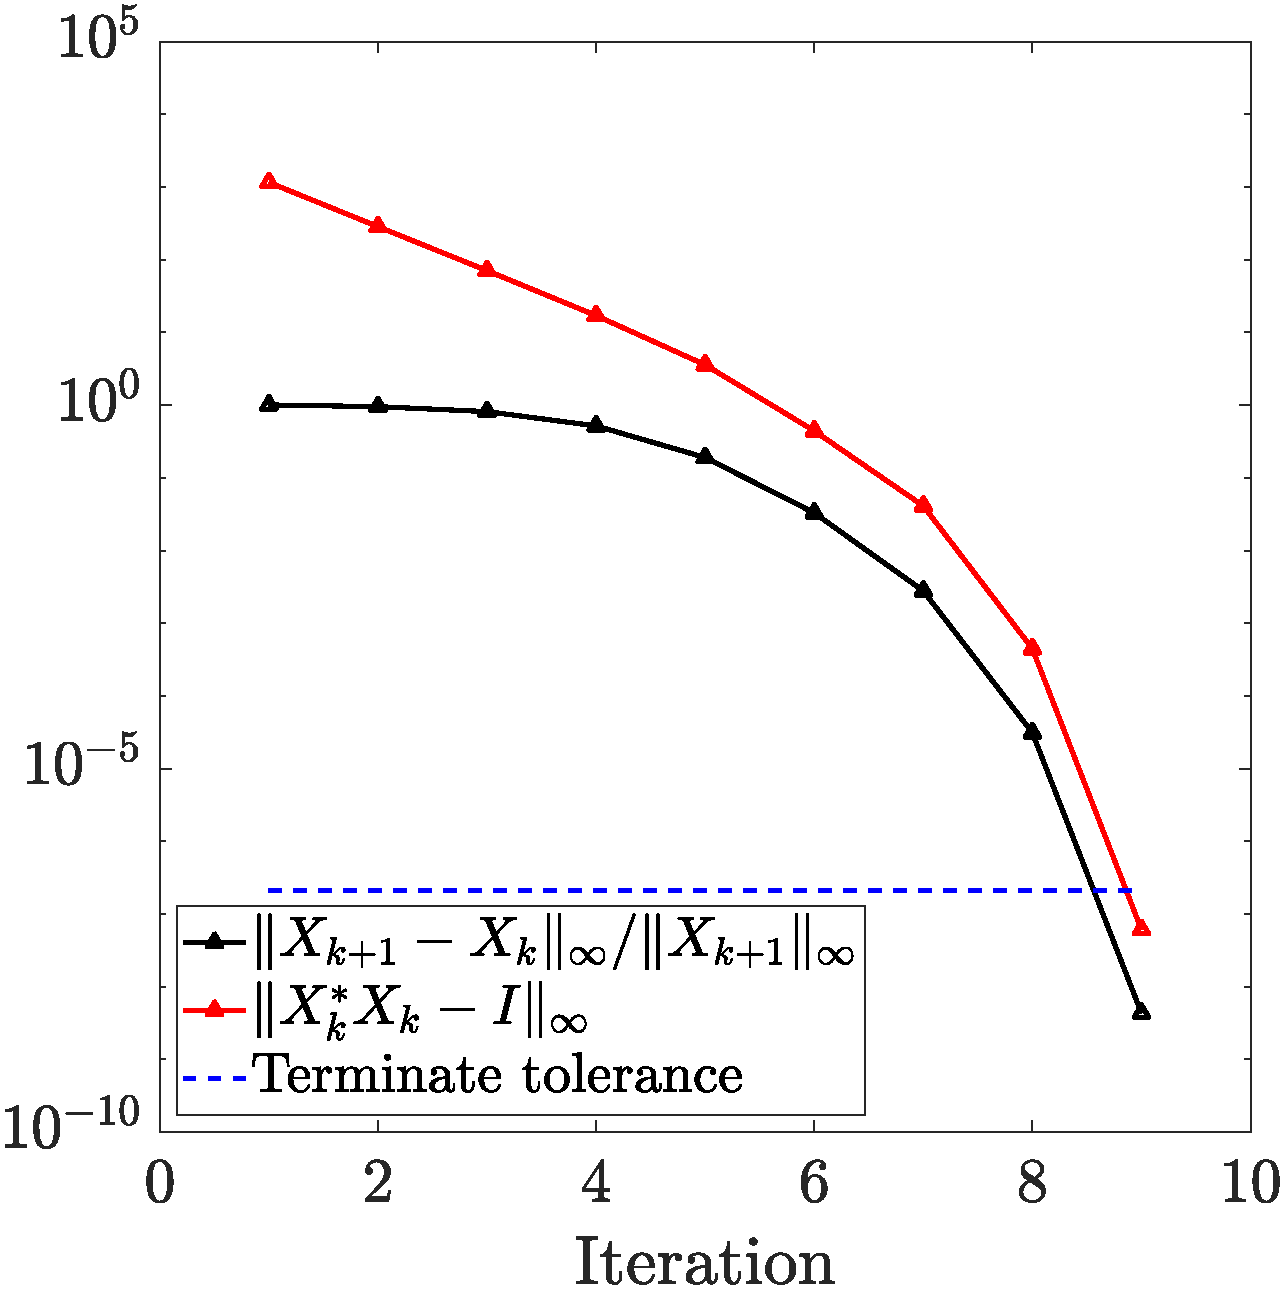
\includegraphics[width=0.6\textwidth]{../code/randn100.pdf}
    \caption{Behaviour of $\gnorm{X_{k+1} - X_{k}}_\infty/\gnorm{X_{k+1}}_\infty$ and $\gnorm{X\ctp X - I}_\infty$ with respect to the iteration when applying \inline{poldec} on \inline{randn(100)}.}
\end{figure}

\begin{figure}[H]
    \centering
    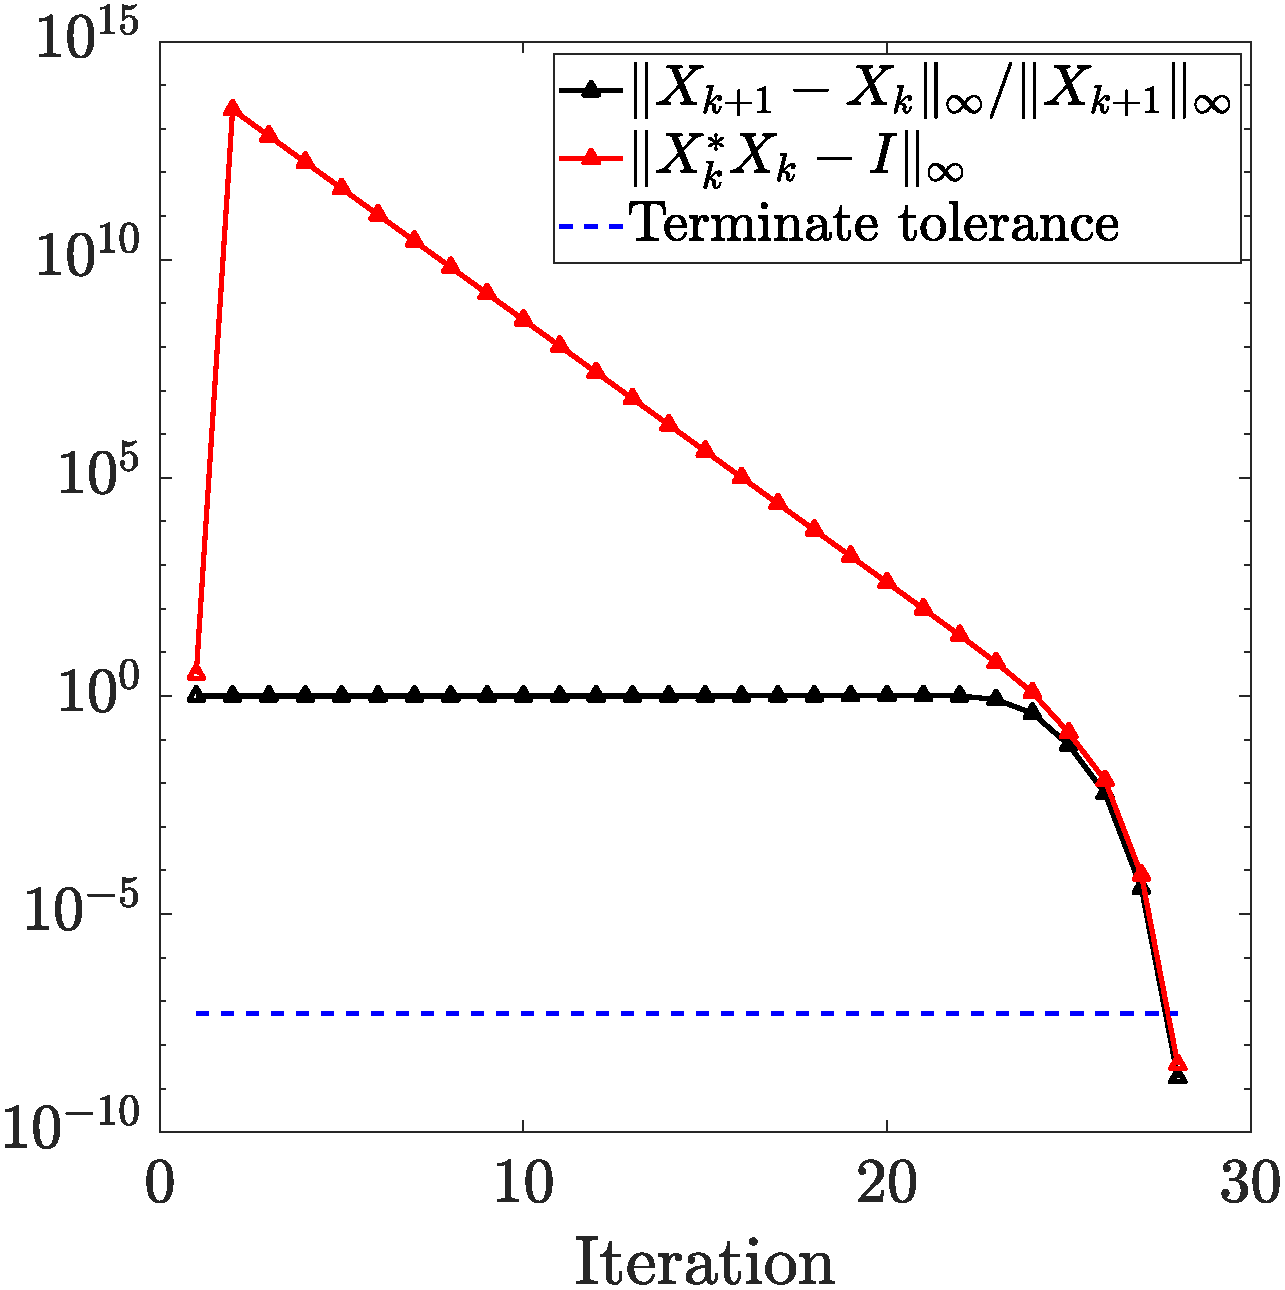
\includegraphics[width=0.6\textwidth]{../code/hilb6.pdf}
    \caption{Behaviour of $\gnorm{X_{k+1} - X_{k}}_\infty/\gnorm{X_{k+1}}_\infty$ and $\gnorm{X\ctp X - I}_\infty$ with respect to the iteration when applying \inline{poldec} on \inline{hilb(6)}.}
    \label{fig:hilb6}
\end{figure}

\begin{figure}[H]
    \centering
    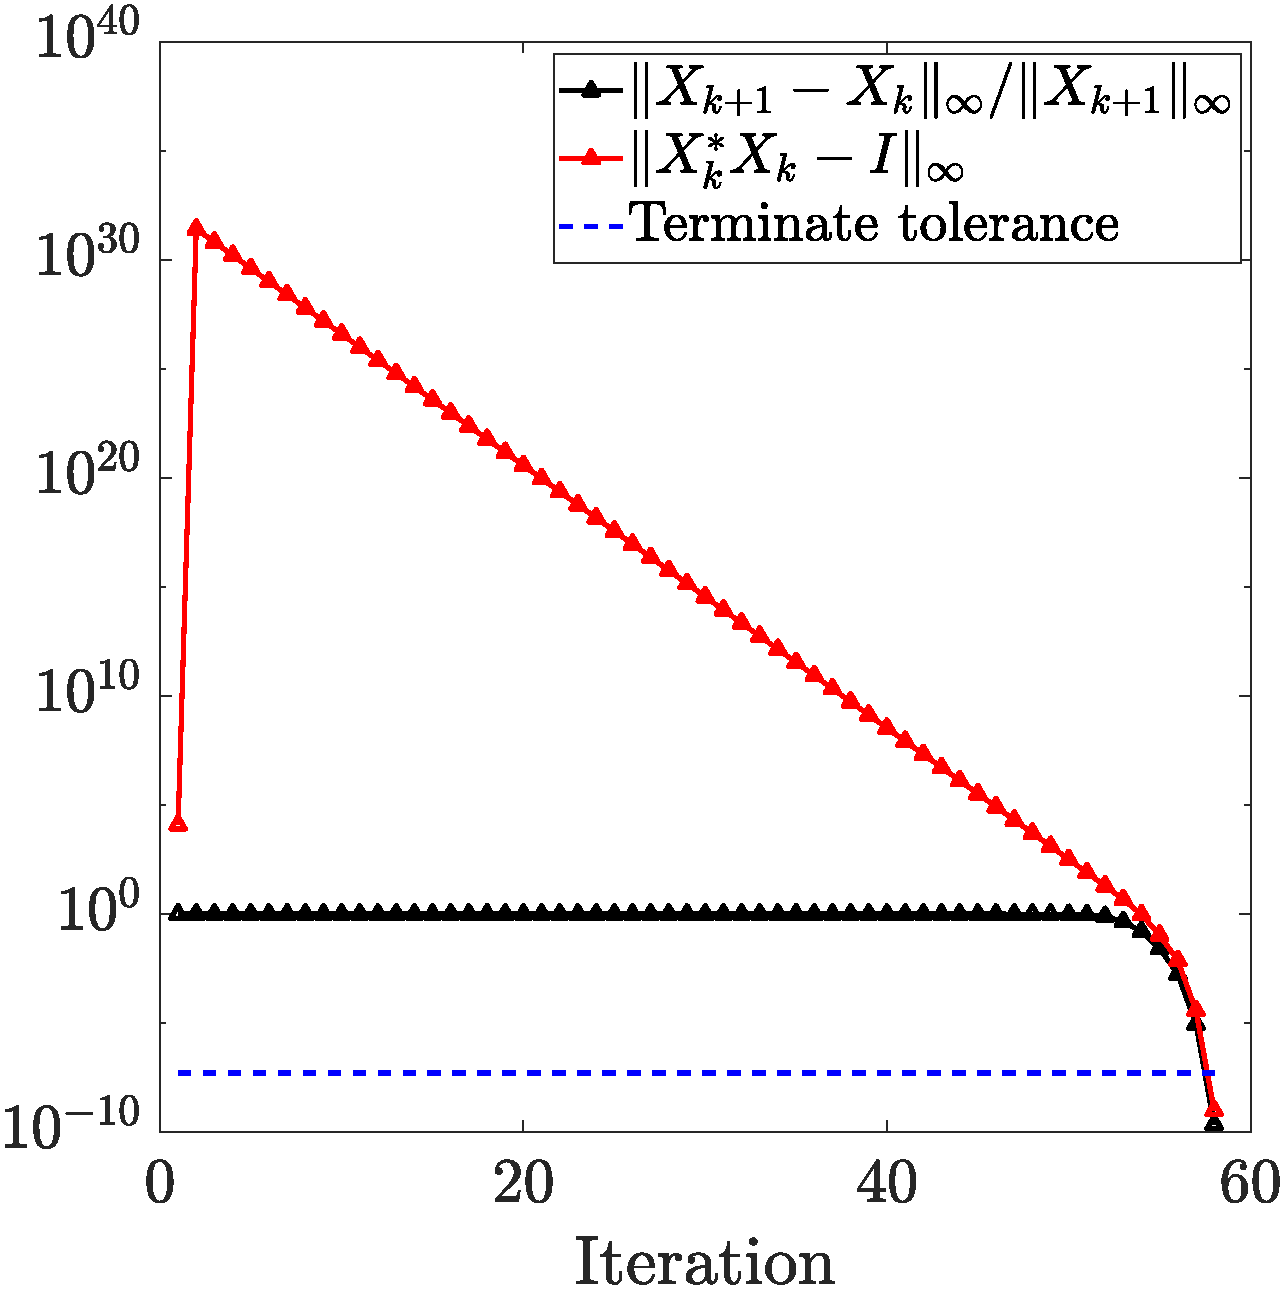
\includegraphics[width=0.6\textwidth]{../code/magic6.pdf}
    \caption{Behaviour of $\gnorm{X_{k+1} - X_{k}}_\infty/\gnorm{X_{k+1}}_\infty$ and $\gnorm{X\ctp X - I}_\infty$ with respect to the iteration when applying \inline{poldec} on \inline{magic(6)}.}
\end{figure}

\begin{figure}[H]
    \centering
    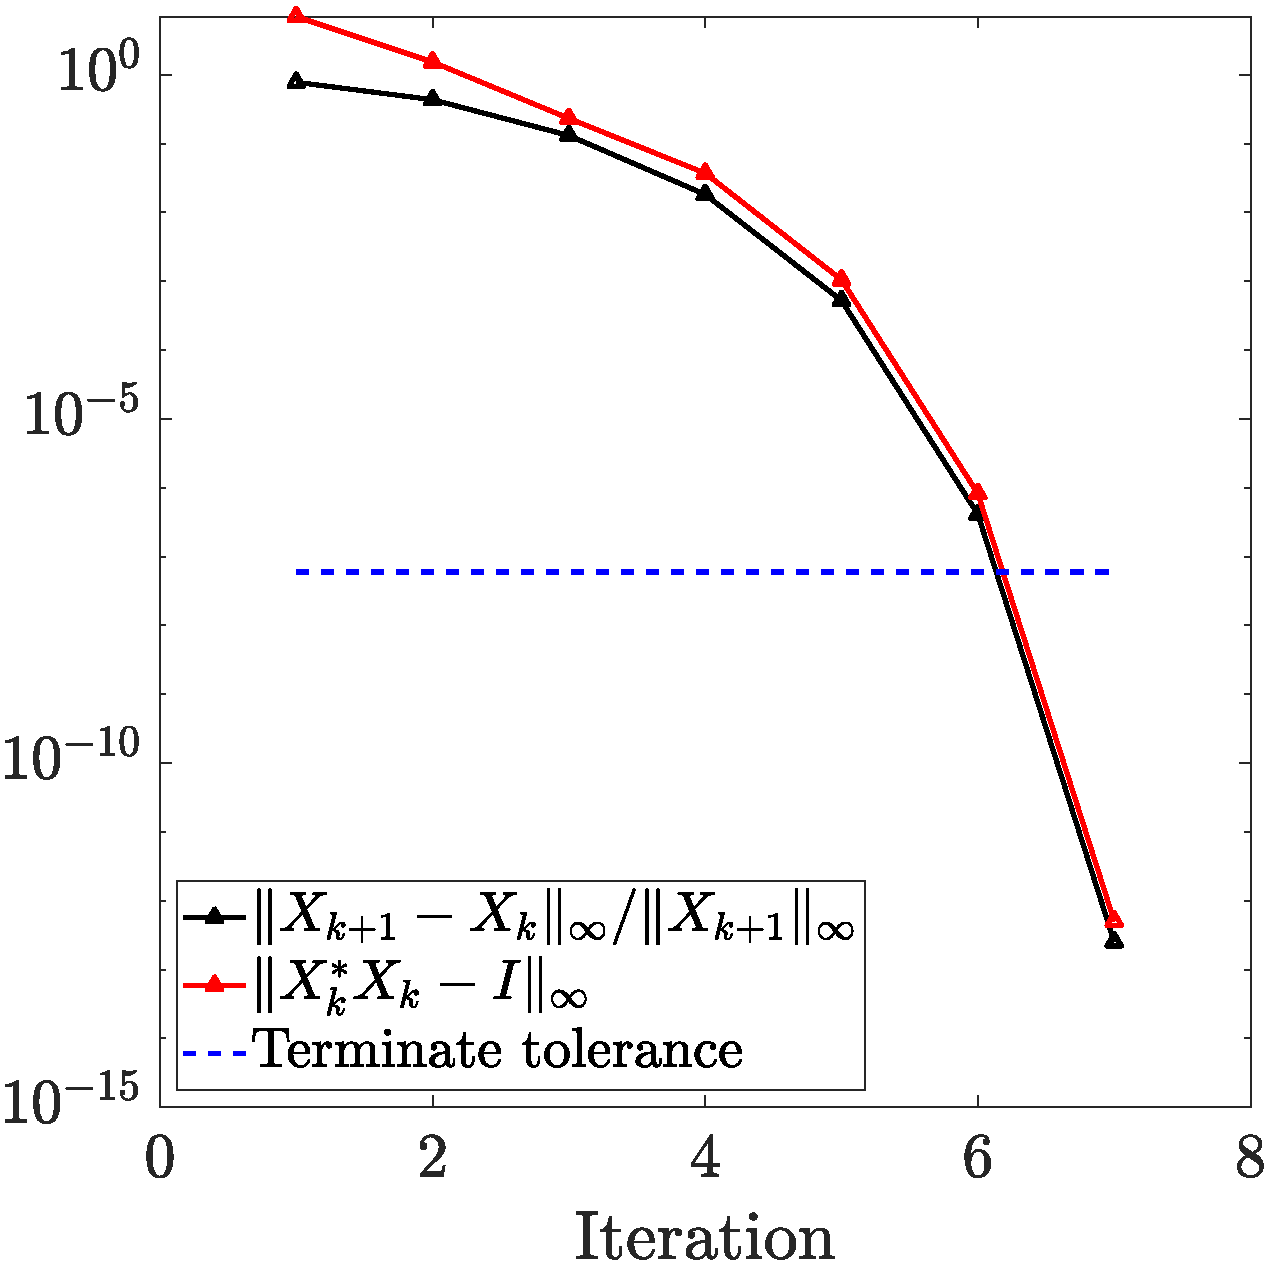
\includegraphics[width=0.6\textwidth]{../code/hadamard8.pdf}
    \caption{Behaviour of $\gnorm{X_{k+1} - X_{k}}_\infty/\gnorm{X_{k+1}}_\infty$ and $\gnorm{X\ctp X - I}_\infty$ with respect to the iteration when applying \inline{poldec} on \inline{hadamard(8)}.}
\end{figure}
